\documentclass{plt}
\usepackage{bbding} % \Checkmark \XsolidBold
\usetheme{metropolis}           % Use metropolis theme

\lstset{
  language=C,
  basicstyle={\fontsize{11}{11.5}\selectfont\ttfamily\spaceskip=3pt},
}


\title{Language Translators}
\author{Ronghui Gu}
\institute{Columbia University}
\date{Spring 2019}
\titlegraphic{
\vspace{230pt}
{\tiny $^*$ These slides are borrowed from Prof. Edwards.}
}
\begin{document}

\frame{\titlepage
}

\begin{frame}[fragile]{What is a Translator?}

A programming language is a notation that  a person and a computer can both understand.
\begin{itemize}

\item It allows you to express what is the \textbf{task} to compute

\item It allows a computer to \textbf{execute} the computation task

\end{itemize}


\alert{A translator translates what you express to what a computer can execute.}

\end{frame}


\begin{frame}[fragile,t]{Compiler}

\begin{center}
\begin{tikzpicture}
  \matrix [matrix of nodes,
           row sep=1pc,
           column sep=2pc,
           every node/.style={draw, fill=white, drop shadow}] {
    & |(a)| Source Program \\
    & |(aa)| Compiler \\
     |(b)| Input &
    |(c)| Machine Code &
    |(d)| Output \\
  };
  \begin{scope}[->]
    \draw (a) -- (aa);
    \draw (aa) -- (c);
    \draw (b) -- (c);
    \draw (c) -- (d);
  \end{scope}
\end{tikzpicture}
\end{center}


\begin{itemize}

\item \textbf{Pros}: translation is done once and for all; 
optimize code and map identifiers at compile time.

\item \textbf{Cons}: long compilation time; hard to port.

\end{itemize}

\end{frame}

\begin{frame}[fragile,t]{Interpreter}

\begin{center}
\begin{tikzpicture}
  \matrix [matrix of nodes,
           row sep=1pc,
           column sep=2pc,
           every node/.style={draw, fill=white, drop shadow}] {
    & |(a)| Source Program \\
     |(b)| Input &
    |(c)| Interpreter &
    |(d)| Output \\
  };
  \begin{scope}[->]
    \draw (a) -- (c);
    \draw (b) -- (c);
    \draw (c) -- (d);
  \end{scope}
\end{tikzpicture}
\end{center}

\begin{itemize}

\item \textbf{Pros}: 
source code distribution; short development cycle.

\item \textbf{Cons}: translation is needed every time a statement is executed;
lack optimization; map identifiers repeatedly.

\end{itemize}

\end{frame}


\begin{frame}[fragile,t]{Bytecode Interpreter}

\begin{center}
\begin{tikzpicture}
  \matrix [matrix of nodes,
           row sep=1pc,
           column sep=2pc,
           every node/.style={draw, fill=white, drop shadow}] {
    & |(a)| Source Program \\
    & |(aa)| Compiler \\
    & |(aaa)| Bytecode \\
     |(b)| Input &
    |(c)| Virtual Machine &
    |(d)| Output \\
  };
  \begin{scope}[->]
    \draw (a) -- (aa);
    \draw (aa) -- (aaa);
    \draw (aaa) -- (c);
    \draw (b) -- (c);
    \draw (c) -- (d);
  \end{scope}
\end{tikzpicture}
\end{center}

\begin{itemize}

\item \textbf{Pros}: bytecode is highly compressed and optimized;
bytecode distribution.

\item \textbf{Cons}: compilation overhead + interpreter overhead.

\end{itemize}

\end{frame}


\begin{frame}[fragile,t]{Just-In-Time Compiler}

\begin{center}
\begin{tikzpicture}
  \matrix [matrix of nodes,
           row sep=1pc,
           column sep=2pc,
           every node/.style={draw, fill=white, drop shadow}] {
    & |(a)| Source Program \\
    & |(aa)| Compiler \\
    & |(aaa)| Bytecode \\
    & |(aaaa)| Just-in-time Compiler \\
     |(b)| Input &
    |(c)| Machine Code &
    |(d)| Output \\
  };
  \begin{scope}[->]
    \draw (a) -- (aa);
    \draw (aa) -- (aaa);
    \draw (aaa) -- (aaaa);
    \draw (aaaa) -- (c);
    \draw (b) -- (c);
    \draw (c) -- (d);
  \end{scope}
  \begin{pgfonlayer}{background}
    \node[draw, fill=yellow!50, inner sep=8pt, fit=(aaaa) (c)] {};
  \end{pgfonlayer}
\end{tikzpicture}

\begin{itemize}

\item \textbf{Pros}: compile and optimize many sections just before the execution;
bytecode distribution.

\item \textbf{Cons}: compilation overhead + warm-up overhead.

\end{itemize}

\end{center}

\end{frame}
%
%\begin{frame}[fragile,t]{Android 4.4 KitKat and earlier}
%
%\begin{center}
%\begin{tikzpicture}
%  \matrix [matrix of nodes,
%           row sep=1pc,
%           column sep=2pc,
%           every node/.style={draw, fill=white, drop shadow}] {
%    & |(a)| Java Source Program \\
%    & |(aa)| Javac Compiler \\
%    & |(aaa)| Java Bytecode \\
%    & |(a4)| dx ``Recompiler'' \\
%    & |(a5)| Dex Bytecode \\
%    & |(a6)| Dalvik Just-in-time Compiler \\
%     |(b)| Input &
%    |(c)| Machine Code &
%    |(d)| Output \\
%  };
%  \begin{scope}[->]
%    \draw (a) -- (aa);
%    \draw (aa) -- (aaa);
%    \draw (aaa) -- (a4);
%    \draw (a4) -- (a5);
%    \draw (a5) -- (a6);
%    \draw (a6) -- (c);
%    \draw (b) -- (c);
%    \draw (c) -- (d);
%  \end{scope}
%  \begin{pgfonlayer}{background}
%    \node[draw, fill=yellow, inner sep=8pt, fit=(a6) (c)] {};
%  \end{pgfonlayer}
%\end{tikzpicture}
%\end{center}
%
%\end{frame}
%
%
%
%\begin{frame}[fragile,t]{Android 5.0 Lollipop}
%
%\begin{center}
%\begin{tikzpicture}
%  \matrix [matrix of nodes,
%           row sep=1pc,
%           column sep=2pc,
%           every node/.style={draw, fill=white, drop shadow}] {
%    & |(a)| Java Source Program \\
%    & |(aa)| Javac Compiler \\
%    & |(aaa)| Java Bytecode \\
%    & |(a4)| dx ``Recompiler'' \\
%    & |(a5)| Dex Bytecode \\
%    & |(a6)| Ahead-of-time Compiler \\
%     |(b)| Input &
%    |(c)| Machine Code &
%    |(d)| Output \\
%  };
%  \begin{scope}[->]
%    \draw (a) -- (aa);
%    \draw (aa) -- (aaa);
%    \draw (aaa) -- (a4);
%    \draw (a4) -- (a5);
%    \draw (a5) -- (a6);
%    \draw (a6) -- (c);
%    \draw (b) -- (c);
%    \draw (c) -- (d);
%  \end{scope}
%\end{tikzpicture}
%\end{center}
%
%\end{frame}



\newcommand{\data}[9]{
  #9
  \draw [line width=1.5pt]
    (-5pc,0) node [anchor=west] {#1} % Label
    ($ln(#3)*(1,0)$) -- ($ln(#4)*(1,0)$) % left whisker
    ($ln(#4)*(1,0)+(0,-2pt)$) [fill] rectangle ($ln(#6)*(1,0)+(0,2pt)$) % box
    ($ln(#6)*(1,0)$) -- ($ln(#7)*(1,0)$) % right whisker
    ;
  \draw [line width=1.5pt,white]
     ($ln(#5)*(1,0)+(0,-2.8pt)$) -- ($ln(#5)*(1,0)+(0,2.8pt)$) % median
  ; \\}
\newcommand{\native}{\color{black!70}}
\newcommand{\jit}{\color{darkgreen!70}}
\newcommand{\bytecode}{\color{red!60}}
\newcommand{\functional}{}
\newcommand{\imperative}{}

\begin{frame}[fragile]{Language Speeds Compared}

\tiny

\begin{tikzpicture}[x=40pt]
  \node [anchor=east] at (0,0) {\native \large Native code compilers};
  \node [anchor=east] at (0,-1pc) {\jit \large Just-in-time compilers};
  \node [anchor=east] at (0,-2pc) {\bytecode \large Bytecode interpreters};
  \matrix [anchor=north east,row sep=0pt,inner sep=0pt] {
	%			min	left	25%	median	75%	right	max
\data{	ATS			}{1.00	}{1.00	}{1.00	}{1.07	}{1.42	}{2.05	}{7.19     }{\native \functional}
\data{	C++ GNU g++		}{1.00	}{1.00	}{1.00	}{1.09	}{1.16	}{1.39	}{1.61     }{\native \imperative}
\data{	C GNU gcc		}{1.00	}{1.00	}{1.00	}{1.11	}{1.21	}{1.53	}{5.19     }{\native \imperative}
\data{	Java 6 steady state	}{1.00	}{1.00	}{1.23	}{1.77	}{1.92	}{2.36	}{2.36     }{\jit \imperative}
\data{	Ada 2005 GNAT		}{1.00	}{1.00	}{1.17	}{2.18	}{4.33	}{8.87	}{8.87     }{\native \imperative}
\data{	Haskell GHC		}{1.00	}{1.00	}{1.59	}{2.26	}{4.80	}{9.63	}{18.38    }{\native \functional}
\data{	Scala			}{1.11	}{1.11	}{1.56	}{2.32	}{4.47	}{6.97	}{6.97     }{\native \imperative}
\data{	Java 6 -server		}{1.08	}{1.08	}{1.64	}{2.34	}{3.87	}{6.80	}{6.80     }{\jit \imperative}
\data{	Lua LuaJIT		}{1.03	}{1.03	}{1.43	}{2.39	}{8.88	}{10.51	}{10.51    }{\jit \imperative}
\data{	Fortran Intel		}{1.00	}{1.00	}{1.65	}{2.76	}{7.74	}{16.87	}{29.54    }{\native \imperative}
%\data{	Clean			}{1.27	}{1.27	}{2.02	}{2.97	}{7.08	}{11.37	}{11.37    }{\native \functional}
\data{	OCaml			}{1.13	}{1.13	}{1.93	}{3.00	}{4.16	}{7.32	}{7.32     }{\native \functional}
\data{	F\# Mono		}{1.65	}{1.65	}{2.07	}{3.21	}{9.68	}{21.11	}{38.05    }{\jit \functional}
\data{	C\# Mono		}{1.58	}{1.58	}{1.95	}{3.33	}{7.24	}{15.17	}{19.06    }{\jit \imperative}
%\data{	Pascal Free Pascal	}{1.61	}{1.61	}{1.89	}{3.49	}{6.18	}{12.61	}{21.84    }{\native \imperative}
\data{	Go 6g 8g		}{1.31	}{1.31	}{2.44	}{3.80	}{13.22	}{29.39	}{126.59   }{\native \imperative}
\data{	Racket			}{1.28	}{1.28	}{2.80	}{4.16	}{8.01	}{15.83	}{20.86    }{\jit \functional}
\data{	Lisp SBCL		}{1.09	}{1.09	}{2.21	}{4.60	}{9.31	}{19.94	}{44.36    }{\native \functional}
\data{	JavaScript V8		}{1.00	}{1.00	}{5.47	}{11.51	}{22.53	}{48.13	}{125.86   }{\jit \imperative}
\data{	Erlang HiPE		}{3.39	}{3.39	}{6.06	}{16.59	}{25.72	}{53.29	}{53.29    }{\jit \functional}
\data{	Lua			}{1.03	}{1.03	}{18.48	}{22.46	}{32.00	}{51.06	}{51.06    }{\bytecode \imperative}
\data{	Smalltalk VisualWorks	}{9.48	}{9.48	}{11.80	}{25.56	}{32.48	}{63.49	}{78.68    }{\bytecode \imperative}
\data{	Java 6 -Xint		}{3.39	}{3.39	}{11.75	}{26.99	}{39.15	}{80.25	}{97.80    }{\bytecode \imperative}
\data{	Python CPython		}{2.28	}{2.28	}{6.04	}{30.33	}{83.78	}{106.47}{106.47   }{\bytecode \imperative}
\data{	Python 3		}{1.97	}{1.97	}{7.32	}{32.13	}{97.40	}{157.73}{157.73   }{\bytecode \imperative}
\data{	Ruby 1.9		}{7.64	}{7.64	}{11.31	}{47.05	}{79.89	}{182.76}{265.59   }{\bytecode \imperative}
\data{	Mozart/Oz		}{7.57	}{7.57	}{32.14	}{50.92	}{85.64	}{165.89}{197.18   }{\bytecode \functional}
%\data{	Ruby JRuby		}{16.33	}{16.33	}{23.17	}{59.88	}{165.92}{380.05}{916.27   }{\bytecode \imperative}
\data{	PHP			}{6.90	}{6.90	}{37.29	}{82.55	}{149.90}{318.81}{491.86   }{\bytecode \imperative}
\data{	Perl			}{2.36	}{2.36	}{6.43	}{88.59	}{193.12}{235.44}{235.44   }{\bytecode \imperative}
%\data{	Ruby MRI		}{15.28	}{15.28	}{20.10	}{138.68}{543.05}{856.12}{856.12   }
};
\end{tikzpicture}

\tiny
Source: http://shootout.alioth.debian.org/
\end{frame}


%%%%%%%%%%%%%%%%%%%%%%%%%%%%%%
\newsavebox{\gcdbox}
\begin{lrbox}{\gcdbox}
\begin{minipage}{0.4\textwidth}
\begin{C}
int avg(int a, int b)
{
  return (a + b) / 2;
}
\end{C}
\end{minipage}
\end{lrbox}
%%%%%%%%%%%%%%%%%%%%%%%%%%%%%%

\part{Compilation Phases}

\tikzset{
    mymodule/.style={draw, fill=white, drop shadow},
    code/.style={draw, fill=gray!15, drop shadow,minimum width=0},
    emph/.style={draw, fill=mBlue!15, drop shadow},
}

\begin{frame}[fragile]{Compiling a Simple Program}
\begin{center}
\hspace{-20pt}
\usebox{\gcdbox}
\end{center}
\vspace{-35pt}
\begin{center}
\begin{tikzpicture}
  \matrix [matrix of nodes,
           row sep=2pc,
           column sep=2pc,
           nodes={mymodule}] {
    |(b)| Compiler \\
    |[code] (c)| 0101110101... \\
  };
  \begin{scope}[->]
    \draw (0pc,4pc) -- (b);
    \draw (b) -- (c);
  \end{scope}
\end{tikzpicture}
\end{center}
\end{frame}




\begin{frame}[fragile,t]{Compilation Phases}

\begin{center}
\hspace{20pt}
\begin{tikzpicture}
  \matrix [matrix of nodes,
           row sep=0.8pc,
           column sep=2pc,
           every node/.style={draw, fill=white, drop shadow,minimum width=5.5cm}] {
     |[code] (b)| int avg (int a, int b) ... \\
     |(a)| Lexical Analysis \\
     |(aa)| Syntax  Analysis \\
     |(aaa)| Semantic Analysis \\
     |(a4)| Intermediate Code Generation \\
     |(a5)| Optimization \\
     |(a6)| Code Generation \\
    |[code] (c)| 0101110101... \\
  };
  \begin{scope}[->]
    \draw (b) -- (a);
    \draw (a) -- (aa);
    \draw (aa) -- (aaa);
    \draw (aaa) -- (a4);
    \draw (a4) -- (a5);
    \draw (a5) -- (a6);
    \draw (a6) -- (c);
  \end{scope};
  \begin{scope}[densely dotted]
    \draw (-10pc,-2.6pc) -- (10pc,-2.6pc);
    \draw (-10pc,-5pc) -- (10pc,-5pc);
  \end{scope};
  \node at (9pc,0) {front-end};
  \node at (9.5pc,-4pc) {middle-end};
  \node at (9pc,-6pc) {back-end};
\end{tikzpicture}
\end{center}

\end{frame}

\begin{frame}[fragile]{What the Compiler Sees}

\usebox{\gcdbox}

\begin{verbatim}
i  n  t SP  a  v  g  (  i  n  t SP  a  , SP  i n  t SP  b  ) NL
{ NL 
SP SP r  e  t  u  r  n SP  ( a SP + SP b ) SP / SP 2 ; NL
} NL
\end{verbatim}

Just a sequence of characters

\end{frame}




\begin{frame}[fragile,t]{Lexical Analysis}

\begin{center}
\hspace{20pt}
\begin{tikzpicture}
  \matrix [matrix of nodes,
           row sep=0.8pc,
           column sep=2pc,
           every node/.style={draw, fill=white, drop shadow,minimum width=5.5cm}] {
     |[code] (b)| int avg (int a, int b) ... \\
     |[emph] (a)| Lexical Analysis \\
     |(aa)| Syntax  Analysis \\
     |(aaa)| Semantic Analysis \\
     |(a4)| Intermediate Code Generation \\
     |(a5)| Optimization \\
     |(a6)| Code Generation \\
    |[code] (c)| 0101110101... \\
  };
  \begin{scope}[->]
    \draw (b) -- (a);
    \draw (a) -- (aa);
    \draw (aa) -- (aaa);
    \draw (aaa) -- (a4);
    \draw (a4) -- (a5);
    \draw (a5) -- (a6);
    \draw (a6) -- (c);
  \end{scope};
  \begin{scope}[densely dotted]
    \draw (-10pc,-2.6pc) -- (10pc,-2.6pc);
    \draw (-10pc,-5pc) -- (10pc,-5pc);
  \end{scope};
  \node at (9pc,0) {front-end};
  \node at (9.5pc,-4pc) {middle-end};
  \node at (9pc,-6pc) {back-end};
\end{tikzpicture}
\end{center}

\end{frame}


%%%%%%%%%%%%%%%%%%%%%%%%%%%%%%

\newcommand{\token}[1]{\tikz \node [minimum height=15pt,draw,rounded corners=2pt,fill=mBlue!10] {#1};}

\def\tokens #1 #2 #3 #4 #5 #6 #7 #8
{\token{#1} 
\token{#2} 
\token{#3} 
\token{#4}
\token{#5} 
\token{#6} 
\token{#7} 
\token{#8}
}

\begin{frame}[fragile]{Lexical Analysis Gives Tokens}
\usebox{\gcdbox}\hfill
%\includegraphics[width=0.45\textwidth]{subway-tokens.jpg}

\renewcommand{\baselinestretch}{2}

{\ttfamily
\tokens int avg ( int a , int b
\tokens ) \{ return ( a + b )
\token{/} \token{2} 
\token{;} \token{\}}\par
}

A stream of tokens.  Whitespace, comments removed.

\end{frame}





\begin{frame}[fragile,t]{Syntax Analysis}

\begin{center}
\hspace{20pt}
\begin{tikzpicture}
  \matrix [matrix of nodes,
           row sep=0.8pc,
           column sep=2pc,
           every node/.style={draw, fill=white, drop shadow,minimum width=5.5cm}] {
     |[code] (b)| int avg (int a, int b) ... \\
     |(a)| Lexical Analysis \\
     |[emph] (aa)| Syntax  Analysis \\
     |(aaa)| Semantic Analysis \\
     |(a4)| Intermediate Code Generation \\
     |(a5)| Optimization \\
     |(a6)| Code Generation \\
    |[code] (c)| 0101110101... \\
  };
  \begin{scope}[->]
    \draw (b) -- (a);
    \draw (a) -- (aa);
    \draw (aa) -- (aaa);
    \draw (aaa) -- (a4);
    \draw (a4) -- (a5);
    \draw (a5) -- (a6);
    \draw (a6) -- (c);
  \end{scope};
  \begin{scope}[densely dotted]
    \draw (-10pc,-2.6pc) -- (10pc,-2.6pc);
    \draw (-10pc,-5pc) -- (10pc,-5pc);
  \end{scope};
  \node at (9pc,0) {front-end};
  \node at (9.5pc,-4pc) {middle-end};
  \node at (9pc,-6pc) {back-end};
\end{tikzpicture}
\end{center}

\end{frame}

\newcommand{\id}[1]{
  node [fill=gray!15] {#1}
}

\newcommand{\theast}{
  \node {func} [level distance=2pc,
    level 1/.style={sibling distance=3.5pc},
    level 2/.style={sibling distance=4.5pc},
    level 3/.style={sibling distance=2.5pc},
    level 4/.style={sibling distance=2.5pc},
    level 5/.style={sibling distance=1.5pc},
  ]
  child {node {int}}
  child {node {avg}}
  child {node {args}
    child {node {arg}
      child {node {int}}
      child {\id a}}
    child {node {arg}
      child {node {int}}
      child {\id b}}
  }
  child [missing]
  child {node {return}
      child {
      	node {/}
      	child {
      		node {+}
      		child {\id a}
      		child {\id b}
      	}
      	child {node {2}}
      }
  }
  ;
}

\begin{frame}
  \frametitle{Syntax Analysis Gives an Abstract Syntax Tree}

\begin{tikzpicture}
  \theast
\end{tikzpicture}

%\vspace{-pc}
\usebox{\gcdbox}

\end{frame}

\renewcommand{\id}[1]{
  node [fill=gray!15] (id) {#1}
  (id) .. controls +(-1,-2) and +(1,0) .. (#1.east)
}

\begin{frame}[fragile,t]{Semantic Analysis}

\begin{center}
\hspace{20pt}
\begin{tikzpicture}
  \matrix [matrix of nodes,
           row sep=0.8pc,
           column sep=2pc,
           every node/.style={draw, fill=white, drop shadow,minimum width=5.5cm}] {
     |[code] (b)| int avg (int a, int b) ... \\
     |(a)| Lexical Analysis \\
     | (aa)| Syntax  Analysis \\
     |[emph] (aaa)| Semantic Analysis \\
     |(a4)| Intermediate Code Generation \\
     |(a5)| Optimization \\
     |(a6)| Code Generation \\
    |[code] (c)| 0101110101... \\
  };
  \begin{scope}[->]
    \draw (b) -- (a);
    \draw (a) -- (aa);
    \draw (aa) -- (aaa);
    \draw (aaa) -- (a4);
    \draw (a4) -- (a5);
    \draw (a5) -- (a6);
    \draw (a6) -- (c);
  \end{scope};
  \begin{scope}[densely dotted]
    \draw (-10pc,-2.6pc) -- (10pc,-2.6pc);
    \draw (-10pc,-5pc) -- (10pc,-5pc);
  \end{scope};
  \node at (9pc,0) {front-end};
  \node at (9.5pc,-4pc) {middle-end};
  \node at (9pc,-6pc) {back-end};
\end{tikzpicture}
\end{center}

\end{frame}

\begin{frame}
  \frametitle{Semantic Analysis: Resolve Symbols; Verify Types}

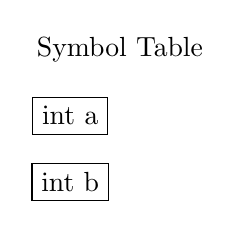
\begin{tikzpicture}
  \node at (-7.5pc, -8pc) {Symbol Table};
  \node [draw] at (-9pc,-10pc) (a) {int a};
  \node [draw] at (-9pc,-12pc) (b) {int b};
  \theast
\end{tikzpicture}

\end{frame}



\begin{frame}[fragile,t]{Intermediate Code Generation}

\begin{center}
\hspace{20pt}
\begin{tikzpicture}
  \matrix [matrix of nodes,
           row sep=0.8pc,
           column sep=2pc,
           every node/.style={draw, fill=white, drop shadow,minimum width=5.5cm}] {
     |[code] (b)| int avg (int a, int b) ... \\
     |(a)| Lexical Analysis \\
     | (aa)| Syntax  Analysis \\
     | (aaa)| Semantic Analysis \\
     |[emph](a4)| Intermediate Code Generation \\
     |(a5)| Optimization \\
     |(a6)| Code Generation \\
    |[code] (c)| 0101110101... \\
  };
  \begin{scope}[->]
    \draw (b) -- (a);
    \draw (a) -- (aa);
    \draw (aa) -- (aaa);
    \draw (aaa) -- (a4);
    \draw (a4) -- (a5);
    \draw (a5) -- (a6);
    \draw (a6) -- (c);
  \end{scope};
  \begin{scope}[densely dotted]
    \draw (-10pc,-2.6pc) -- (10pc,-2.6pc);
    \draw (-10pc,-5pc) -- (10pc,-5pc);
  \end{scope};
  \node at (9pc,0) {front-end};
  \node at (9.5pc,-4pc) {middle-end};
  \node at (9pc,-6pc) {back-end};
\end{tikzpicture}
\end{center}

\end{frame}

%%%%%%%%%%%%%%%%%%%%%%%%%%%%%%

\begin{frame}[fragile]
  \frametitle{Translation into 3-Address Code}


\usebox{\gcdbox}\hfill\parbox{20pc}{\raggedright
Idealized assembly language w/ infinite registers
}

\begin{assembly}
avg: 
  t0 := a + b
  t1 := 2
  t2 := t0 / t1
  ret t2	
\end{assembly}
% Generated from SUIF/MachSUIF:
%
% c2s gcd.c
% do_lower gcd.suif gcd.lsuif
% do_s2m gcd.lsuif gcd.suifvm
% do_print gcd.suifvm
%
% Heavily massaged to make it readable

\end{frame}



\begin{frame}[fragile,t]{Optimization}

\begin{center}
\hspace{20pt}
\begin{tikzpicture}
  \matrix [matrix of nodes,
           row sep=0.8pc,
           column sep=2pc,
           every node/.style={draw, fill=white, drop shadow,minimum width=5.5cm}] {
     |[code] (b)| int avg (int a, int b) ... \\
     |(a)| Lexical Analysis \\
     | (aa)| Syntax  Analysis \\
     | (aaa)| Semantic Analysis \\
     |(a4)| Intermediate Code Generation \\
     |[emph](a5)| Optimization \\
     |(a6)| Code Generation \\
    |[code] (c)| 0101110101... \\
  };
  \begin{scope}[->]
    \draw (b) -- (a);
    \draw (a) -- (aa);
    \draw (aa) -- (aaa);
    \draw (aaa) -- (a4);
    \draw (a4) -- (a5);
    \draw (a5) -- (a6);
    \draw (a6) -- (c);
  \end{scope};
  \begin{scope}[densely dotted]
    \draw (-10pc,-2.6pc) -- (10pc,-2.6pc);
    \draw (-10pc,-5pc) -- (10pc,-5pc);
  \end{scope};
  \node at (9pc,0) {front-end};
  \node at (9.5pc,-4pc) {middle-end};
  \node at (9pc,-6pc) {back-end};
\end{tikzpicture}
\end{center}

\end{frame}


\begin{frame}[fragile]
  \frametitle{Optimization}


\begin{center}
\begin{tikzpicture}
  \matrix [matrix of nodes,
           row sep=0.8pc,
           column sep=2pc,
           every node/.style={draw, fill=white, drop shadow,minimum width=5.5cm}] {
     |[emph](a)| Optimization \\
  };
  \begin{scope}[->]
    \draw (0pc,2.5pc) -- (a);
    \draw (a) -- (0pc,-2.4pc) ;
  \end{scope};
  \node at (0pc,2.5) {\begin{assembly}
avg: 
  t0 := a + b
  t1 := 2
  t2 := t0 / t1
  ret t2	
\end{assembly}};
  \node at (0pc,-5pc) {\begin{assembly}
avg: 
  t0 := a + b
  t2 := t0 / 2
  ret t2	
\end{assembly}};
\end{tikzpicture}
\end{center}

% Generated from SUIF/MachSUIF:
%
% c2s gcd.c
% do_lower gcd.suif gcd.lsuif
% do_s2m gcd.lsuif gcd.suifvm
% do_print gcd.suifvm
%
% Heavily massaged to make it readable

\end{frame}


\begin{frame}[fragile,t]{Code Generation}

\begin{center}
\hspace{20pt}
\begin{tikzpicture}
  \matrix [matrix of nodes,
           row sep=0.8pc,
           column sep=2pc,
           every node/.style={draw, fill=white, drop shadow,minimum width=5.5cm}] {
     |[code] (b)| int avg (int a, int b) ... \\
     |(a)| Lexical Analysis \\
     | (aa)| Syntax  Analysis \\
     | (aaa)| Semantic Analysis \\
     |(a4)| Intermediate Code Generation \\
     |(a5)| Optimization \\
     |[emph] (a6)| Code Generation \\
    |[code] (c)| 0101110101... \\
  };
  \begin{scope}[->]
    \draw (b) -- (a);
    \draw (a) -- (aa);
    \draw (aa) -- (aaa);
    \draw (aaa) -- (a4);
    \draw (a4) -- (a5);
    \draw (a5) -- (a6);
    \draw (a6) -- (c);
  \end{scope};
  \begin{scope}[densely dotted]
    \draw (-10pc,-2.6pc) -- (10pc,-2.6pc);
    \draw (-10pc,-5pc) -- (10pc,-5pc);
  \end{scope};
  \node at (9pc,0) {front-end};
  \node at (9.5pc,-4pc) {middle-end};
  \node at (9pc,-6pc) {back-end};
\end{tikzpicture}
\end{center}

\end{frame}
%%%%%%%%%%%%%%%%%%%%%%%%%%%%%%

\begin{frame}[fragile]{Generation of x86 Assembly}


\begin{center}
\begin{tikzpicture}
  \matrix [matrix of nodes,
           row sep=0.8pc,
           column sep=2pc,
           every node/.style={draw, fill=white, drop shadow,minimum width=5.5cm}] {
     |[emph](a)| Code Generation \\
  };
  \begin{scope}[->]
    \draw (0pc,2.5pc) -- (a);
    \draw (a) -- (0pc,-1.5pc) ;
  \end{scope};
  \node at (0pc,1.7) {\begin{assembly}
avg: 
  t0 := a + b
  t2 := t0 / 2
  ret t2	
\end{assembly}};
  \node at (0pc,-6.5pc) {\begin{assembly}
avg:  pushl %ebp          # save BP
      movl  %esp,%ebp
      movl  8(%ebp),%eax  # load a from stack
      movl  12(%ebp),%edx # load b from stack
      
      addl  %edx,%eax     # a += b
      shr   $1,%eax       # a /= 2
      ret
\end{assembly}};
\end{tikzpicture}
\end{center}


%\raisebox{2pc}{\scalebox{0.75}{\usebox{\gcdbox}}}\hfill \includegraphics[width=5pc]{80386.jpg}


\end{frame}

\end{document}

% Local Variables:
% compile-command: "make processors.pdf"
% End:

